\documentclass{standalone}
\usepackage{tikz}
\usetikzlibrary{patterns, positioning}
\usetikzlibrary{shapes.misc}
\usepackage[outline]{contour}
\contourlength{1.5pt} 
\usepackage[sfdefault]{ClearSans} %% option 'sfdefault' activates Clear Sans as the default text font
\usepackage[T1]{fontenc}

\begin{document}
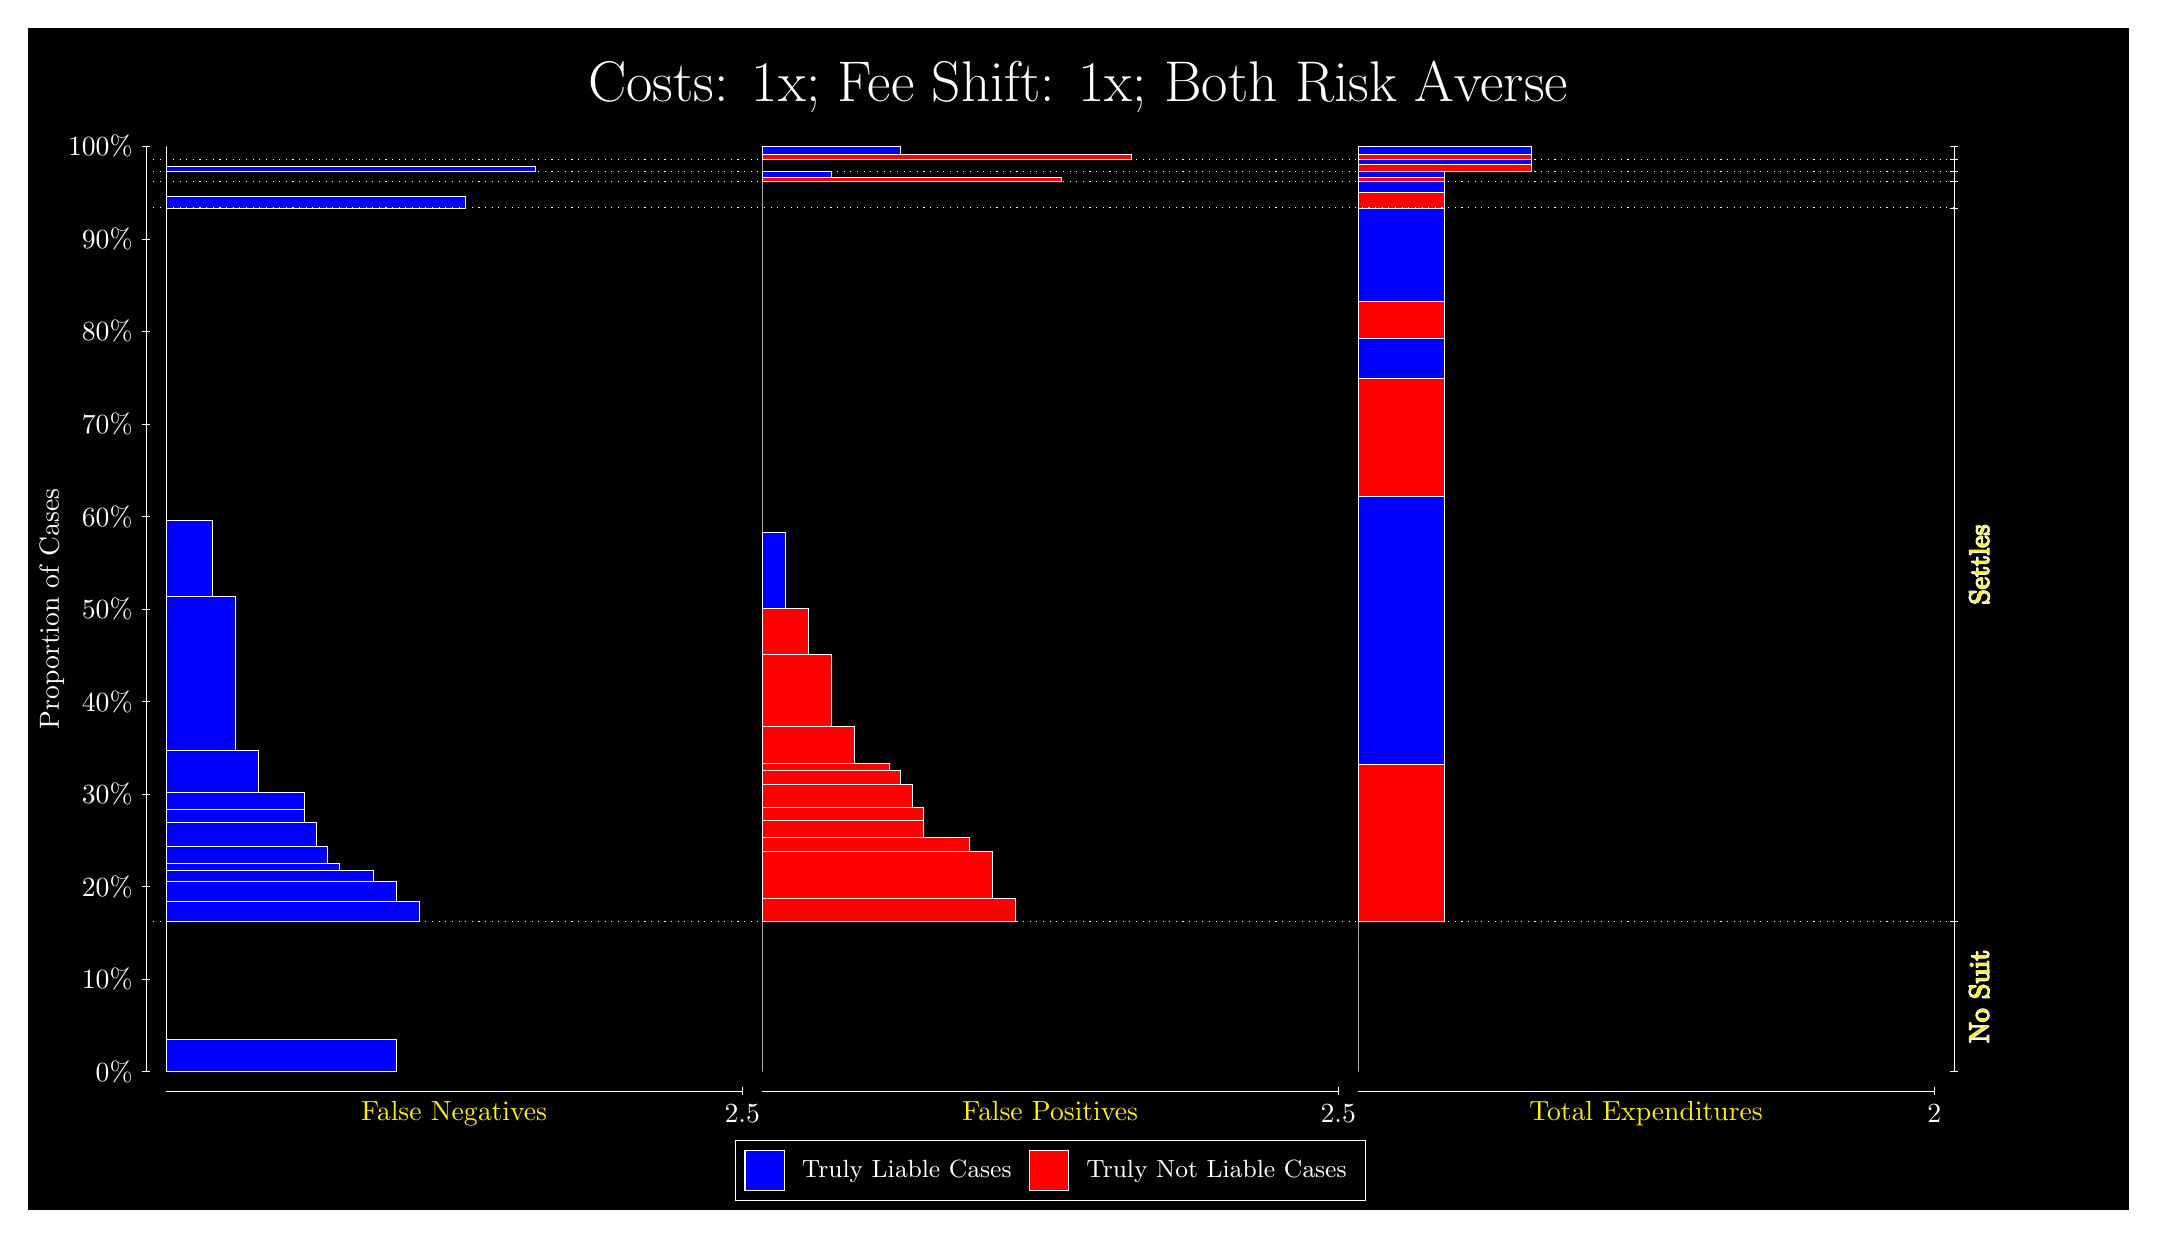
\begin{tikzpicture}
\draw[fill=black] (0,0) rectangle (26.667,15);
\draw[text=white] (0,13.5) rectangle (26.667,15) node[midway] {\huge Costs: 1x; Fee Shift: 1x; Both Risk Averse};
\draw[white, very thin] (1.5,1.75) -- (1.5,13.5);
\node[rotate=90, text=white, anchor=center] at (0.3, 7.625) {Proportion of Cases};
\draw[white, very thin] (1.45,1.75) -- (1.55,1.75);
\node[text=white, anchor=east] at (1.45, 1.75) {0\%};
\draw[white, very thin] (1.45,2.925) -- (1.55,2.925);
\node[text=white, anchor=east] at (1.45, 2.925) {10\%};
\draw[white, very thin] (1.45,4.1) -- (1.55,4.1);
\node[text=white, anchor=east] at (1.45, 4.1) {20\%};
\draw[white, very thin] (1.45,5.275) -- (1.55,5.275);
\node[text=white, anchor=east] at (1.45, 5.275) {30\%};
\draw[white, very thin] (1.45,6.45) -- (1.55,6.45);
\node[text=white, anchor=east] at (1.45, 6.45) {40\%};
\draw[white, very thin] (1.45,7.625) -- (1.55,7.625);
\node[text=white, anchor=east] at (1.45, 7.625) {50\%};
\draw[white, very thin] (1.45,8.8) -- (1.55,8.8);
\node[text=white, anchor=east] at (1.45, 8.8) {60\%};
\draw[white, very thin] (1.45,9.975) -- (1.55,9.975);
\node[text=white, anchor=east] at (1.45, 9.975) {70\%};
\draw[white, very thin] (1.45,11.15) -- (1.55,11.15);
\node[text=white, anchor=east] at (1.45, 11.15) {80\%};
\draw[white, very thin] (1.45,12.325) -- (1.55,12.325);
\node[text=white, anchor=east] at (1.45, 12.325) {90\%};
\draw[white, very thin] (1.45,13.5) -- (1.55,13.5);
\node[text=white, anchor=east] at (1.45, 13.5) {100\%};

\draw[white, very thin] (24.457,1.75) -- (24.457,13.5);
\draw[white, very thin] (24.407,1.75) -- (24.507,1.75);
\node[anchor=west] at (24.407, 1.75) {};
\draw[white, very thin] (24.407,3.6589) -- (24.507,3.6589);
\node[anchor=west] at (24.407, 3.6589) {};
\draw[white, very thin] (24.407,12.718) -- (24.507,12.718);
\node[anchor=west] at (24.407, 12.718) {};
\draw[white, very thin] (24.407,13.057) -- (24.507,13.057);
\node[anchor=west] at (24.407, 13.057) {};
\draw[white, very thin] (24.407,13.183) -- (24.507,13.183);
\node[anchor=west] at (24.407, 13.183) {};
\draw[white, very thin] (24.407,13.334) -- (24.507,13.334);
\node[anchor=west] at (24.407, 13.334) {};
\draw[white, very thin] (24.407,13.5) -- (24.507,13.5);
\node[anchor=west] at (24.407, 13.5) {};

\draw[white, very thin, fill=blue] (1.75,1.75) rectangle (4.6775,2.1593);
\draw[white, very thin, fill=red] (1.75,2.1593) rectangle (1.75,3.6589);
\draw[white, very thin, fill=blue] (1.75,3.6589) rectangle (4.9703,3.9069);
\draw[white, very thin, fill=blue] (1.75,3.9069) rectangle (4.6775,4.1689);
\draw[white, very thin, fill=blue] (1.75,4.1689) rectangle (4.3848,4.3003);
\draw[white, very thin, fill=blue] (1.75,4.3003) rectangle (3.9457,4.3942);
\draw[white, very thin, fill=blue] (1.75,4.3942) rectangle (3.7993,4.6081);
\draw[white, very thin, fill=blue] (1.75,4.6081) rectangle (3.6529,4.9144);
\draw[white, very thin, fill=blue] (1.75,4.9144) rectangle (3.5065,5.0771);
\draw[white, very thin, fill=blue] (1.75,5.0771) rectangle (3.5065,5.2922);
\draw[white, very thin, fill=blue] (1.75,5.2922) rectangle (2.921,5.8301);
\draw[white, very thin, fill=blue] (1.75,5.8301) rectangle (2.6283,7.781);
\draw[white, very thin, fill=blue] (1.75,7.781) rectangle (2.3355,8.7493);
\draw[white, very thin, fill=red] (1.75,8.7493) rectangle (1.75,12.718);
\draw[white, very thin, fill=blue] (1.75,12.718) rectangle (5.5558,12.86);
\draw[white, very thin, fill=red] (1.75,12.86) rectangle (1.75,13.057);
\draw[white, very thin, fill=red] (1.75,13.057) rectangle (1.75,13.113);
\draw[white, very thin, fill=blue] (1.75,13.113) rectangle (1.75,13.183);
\draw[white, very thin, fill=blue] (1.75,13.183) rectangle (6.4341,13.246);
\draw[white, very thin, fill=red] (1.75,13.246) rectangle (1.75,13.334);
\draw[white, very thin, fill=red] (1.75,13.334) rectangle (1.75,13.399);
\draw[white, very thin, fill=blue] (1.75,13.399) rectangle (1.75,13.5);
\draw[white, very thin, fill=red] (9.3189,1.75) rectangle (9.3189,3.2496);
\draw[white, very thin, fill=blue] (9.3189,3.2496) rectangle (9.3189,3.6589);
\draw[white, very thin, fill=red] (9.3189,3.6589) rectangle (12.539,3.9507);
\draw[white, very thin, fill=red] (9.3189,3.9507) rectangle (12.246,4.5449);
\draw[white, very thin, fill=red] (9.3189,4.5449) rectangle (11.954,4.7243);
\draw[white, very thin, fill=red] (9.3189,4.7243) rectangle (11.368,4.9394);
\draw[white, very thin, fill=red] (9.3189,4.9394) rectangle (11.368,5.1058);
\draw[white, very thin, fill=red] (9.3189,5.1058) rectangle (11.222,5.3995);
\draw[white, very thin, fill=red] (9.3189,5.3995) rectangle (11.075,5.5818);
\draw[white, very thin, fill=red] (9.3189,5.5818) rectangle (10.929,5.6706);
\draw[white, very thin, fill=red] (9.3189,5.6706) rectangle (10.49,6.129);
\draw[white, very thin, fill=red] (9.3189,6.129) rectangle (10.197,7.0461);
\draw[white, very thin, fill=red] (9.3189,7.0461) rectangle (9.9044,7.6281);
\draw[white, very thin, fill=blue] (9.3189,7.6281) rectangle (9.6116,8.5964);
\draw[white, very thin, fill=blue] (9.3189,8.5964) rectangle (9.3189,12.718);
\draw[white, very thin, fill=red] (9.3189,12.718) rectangle (9.3189,12.916);
\draw[white, very thin, fill=blue] (9.3189,12.916) rectangle (9.3189,13.057);
\draw[white, very thin, fill=red] (9.3189,13.057) rectangle (13.125,13.113);
\draw[white, very thin, fill=blue] (9.3189,13.113) rectangle (10.197,13.183);
\draw[white, very thin, fill=red] (9.3189,13.183) rectangle (9.3189,13.271);
\draw[white, very thin, fill=blue] (9.3189,13.271) rectangle (9.3189,13.334);
\draw[white, very thin, fill=red] (9.3189,13.334) rectangle (14.003,13.399);
\draw[white, very thin, fill=blue] (9.3189,13.399) rectangle (11.075,13.5);
\draw[white, very thin, fill=red] (16.888,1.75) rectangle (16.888,3.2496);
\draw[white, very thin, fill=blue] (16.888,3.2496) rectangle (16.888,3.6589);
\draw[white, very thin, fill=red] (16.888,3.6589) rectangle (17.986,5.655);
\draw[white, very thin, fill=blue] (16.888,5.655) rectangle (17.986,9.0532);
\draw[white, very thin, fill=red] (16.888,9.0532) rectangle (17.986,10.552);
\draw[white, very thin, fill=blue] (16.888,10.552) rectangle (17.986,11.062);
\draw[white, very thin, fill=red] (16.888,11.062) rectangle (17.986,11.536);
\draw[white, very thin, fill=blue] (16.888,11.536) rectangle (17.986,12.718);
\draw[white, very thin, fill=red] (16.888,12.718) rectangle (17.986,12.916);
\draw[white, very thin, fill=blue] (16.888,12.916) rectangle (17.986,13.057);
\draw[white, very thin, fill=red] (16.888,13.057) rectangle (17.986,13.113);
\draw[white, very thin, fill=blue] (16.888,13.113) rectangle (17.986,13.183);
\draw[white, very thin, fill=red] (16.888,13.183) rectangle (19.083,13.271);
\draw[white, very thin, fill=blue] (16.888,13.271) rectangle (19.083,13.334);
\draw[white, very thin, fill=red] (16.888,13.334) rectangle (19.083,13.399);
\draw[white, very thin, fill=blue] (16.888,13.399) rectangle (19.083,13.5);
\draw[white, dotted] (1.5,3.6589) -- (24.457,3.6589);
\draw[white, dotted] (1.5,12.718) -- (24.457,12.718);
\draw[white, dotted] (1.5,13.057) -- (24.457,13.057);
\draw[white, dotted] (1.5,13.183) -- (24.457,13.183);
\draw[white, dotted] (1.5,13.334) -- (24.457,13.334);
\draw[white, very thin] (1.75,1.5) -- (9.0689,1.5);
\node[text=yellow, anchor=north] at (5.4094, 1.5) {False Negatives};
\draw[white, very thin] (9.0689,1.45) -- (9.0689,1.55);
\node[text=white, anchor=north] at (9.0689, 1.45) {2.5};

\draw[white, very thin] (9.3189,1.5) -- (16.638,1.5);
\node[text=yellow, anchor=north] at (12.978, 1.5) {False Positives};
\draw[white, very thin] (16.638,1.45) -- (16.638,1.55);
\node[text=white, anchor=north] at (16.638, 1.45) {2.5};

\draw[white, very thin] (16.888,1.5) -- (24.207,1.5);
\node[text=yellow, anchor=north] at (20.547, 1.5) {Total Expenditures};
\draw[white, very thin] (24.207,1.45) -- (24.207,1.55);
\node[text=white, anchor=north] at (24.207, 1.45) {2};

\node[text=yellow, centered, rotate=90] at (24.777, 2.7045) {\contour{white}{No Suit}};
\node[text=yellow, centered, rotate=90] at (24.777, 8.1887) {\contour{white}{Settles}};





\draw (12.978300999999998,1.5) node[draw=none] (baseCoordinate) {};
\begin{scope}[align=center]
        \matrix[scale=0.5, draw=white, below=0.5cm of baseCoordinate, nodes={draw}, column sep=0.1cm]{
            \node[rectangle, draw, minimum width=0.5cm, minimum height=0.5cm, fill=blue] {}; &
            \node[draw=none, font=\small, text=white] (B) {Truly Liable Cases}; &
            \node[rectangle, draw, minimum width=0.5cm, minimum height=0.5cm, fill=red] {}; &
            \node[draw=none, font=\small, text=white] (B) {Truly Not Liable Cases}; \\
            };
\end{scope}

\end{tikzpicture}
\end{document}